\setcounter{ExampleCounter}{1}

This is one of the most fundamental topics in all of algebra.  In fact, this is the kind of algebra that you likely do all the time without realizing it.  For instance, if someone tells you the time by saying, ``It's a quarter to 3,'' what they're really saying is ``take the time that it is now, add 15 minutes to it, and you'll end up at 3 o'clock.''  You automatically figure out that it must be 2:45, but what you've really done is solve the following equation: \[x + \textrm{0:15} = \textrm{3:00}\] where $x$ represents the time that it is now.\\

Here's another example: suppose you are on a long drive, and your GPS tells you that you're 50 miles away from Disneyland.  If you're driving 75 miles per hour, how long will it take you to get there?

To find the equation for this one, we need to know a relationship between speed and distance traveled.  Your hint is the units for speed: \textbf{miles \emph{per} hour}.  This means that each hour, you travel 75 miles.  Thus, the distance that you travel is 75 times the number of hours that go by:
\[\textrm{Distance } = \left(75\ \dfrac{mi}{hr}\right) (x \ hr)\marginnote{Notice that the hours cancel when you multiply those\\ units, leaving miles.  This is\\ a good confirmation that\\ you've set up the equation\\ correctly.}\]
Therefore, if we know the distance we want to travel (50 mi), we can plug that in for distance:
\[75x = 50\]
By solving this equation for $x$, we can find the amount of time it will take to cover this distance.

\paragraph{Solving Equations} Of course, these are fairly straightforward to solve; we'd like to be able to handle more complicated situations.  The principles that we see in this section, though, will hold for the complicated ones as well as the simple ones.  To \textbf{solve} an equation means to find the value for the variable that will make the equation work correctly.\\

In other words, for the example with the speed above, if we solved the equation (using the methods we'll see a bit later), we would find that the time remaining is 2/3 hr (or 40 minutes).  We can be confident that this is the right answer, because if we replace $x$ with 2/3, it makes the equation true:
\[75\left(\dfrac{2}{3}\right) = 50\]
You can check this result on your calculator, but it is true.\\

By the way, this kind of checking is always a good idea when you finish solving an equation.  You can catch lots of small mistakes by plugging your answer back into the equation at the end to verify that it works.\\

How, then, do we actually solve an equation?  There is one crucial principle that you need to remember; if you understand this, you can learn how to solve any type of equation.

\begin{proc}{Solving Equations}
The key to solving equations:
\begin{center}
Whatever\marginnote{
\includegraphics[width=1.25in]{Balance}} you do to one side of an equation, you must do to the other side.
\end{center}

You can think of an equation like a balance scale (as shown in the margin).  An equation just says ``this thing on the left-hand side is equal to this thing on the right-hand side.''  Therefore, if we, say, add 5 to both sides, the equation will still balance.\\

To solve any kind of equation, then, we just have to figure out what operations we need to carry out in order to get $x$ by itself on one side of the equation, and do those operations to both sides at the same time.
\end{proc}
\pagebreak

\subsection{Solving Linear Equations}
A linear equation with one variable looks like the following examples:
\begin{align*}
x + 3 &= 17\\
2x &= 9\\
4x - 5 &= -6\\
3 &= 5-y\\
z+1 &= 2z-3
\end{align*}

We can write these in many different ways, but notice how all of these examples have one variable in each of them (whether that is $x$, $y$, $z$, or any other letter that we want to use).  Furthermore, that variable is at most multiplied by a number (like $2x$ in the second example); there are no exponents (like $x^2$, which we'll see later in this section).  Finally, something may be added to or subtracted from that variable piece (like $4x-5$ in the third example).\\

\begin{example}{Solving Linear Equations}
Solve the following equation:
\[x + 3 = 7\]

\sol
You may be able to see the answer to this one, but let's think about how we can solve it systematically.  We want to have $x$ by itself on one side of the equation at the end, so what is it that's stopping that from being the case?  The answer is that there is a 3 being added to $x$.\\

To get rid of this 3 (which is added), we will \emph{subtract} 3.  Remember, we're allowed to do this as long as we do the same thing to the other side of the equation:
\begin{alignat*}{3}
x\ +\ &3\ &&=\ &&7\\
{\color{red}-}&{\color{red}3}\ &&\ &&{\color{red}-3}\\
&x &&=\ &&\boxed{4}
\end{alignat*}
\end{example}

\begin{example}{Solving Linear Equations}
Solve the following equation:
\[x - 5 = -2\]

\sol
For this one, we notice that the only thing stopping $x$ from being by itself is the $-5$, which we can remove by \emph{adding} 5 to both sides of the equation:\
\begin{alignat*}{3}
x\ -\ &5\ &&=\ &&-2\\
{\color{red}+}&{\color{red}5}\ &&\ &&{\color{red}+5}\\
&x &&=\ &&\boxed{3}
\end{alignat*}

Remember,\marginnote{\bfseries Check} we can check this answer by plugging it back into the original equation:
\[3 - 5 = 2\]  This is a true statement, so our answer checks out.
\end{example}

\begin{proc}{Addition Principle}
Some books call what we've just done the \textbf{Addition Principle}, which states that we can add or subtract anything we want to/from each side of an equation, and the equation will still be true (the scales will still be balanced).\\

To write this statement in symbolic terms, we could say that if we have an equation \[a = b\] where $a$ and $b$ are simply placeholders for whatever is written on each side of the equation, we can add $c$ (any number, known or unknown) to both sides: \[a + c = b + c\]

Of course, the Addition Principle is just one application of the general principle stated above, that we can do \emph{any} operation we like to one side of an equation, as long as we do the same to the other side.
\end{proc}

\begin{example}{Solving Linear Equations}
Solve the following equation:
\[3x = 9\]

\sol
Now to get $x$ by itself, we must \emph{divide} both sides by 3, because $x$ is being multiplied by 3 (we do the opposite--division--to get rid of the 3).
\begin{align*}
3x &= 9\\
\dfrac{3x}{3} &= \dfrac{9}{3}\\
x &= \boxed{3}
\end{align*}
\end{example}

\begin{example}{Solving Linear Equations}
Solve the following equation:
\[\dfrac{x}{4} = 5\]

\sol
This one involves dividing $x$ by something, so to undo that, we'll need to \emph{multiply} $x$ by that thing (4 in this case).
\begin{align*}
\dfrac{x}{4} &= 5\\
(4) \left(\dfrac{x}{4}\right) &= (5) (4)\\
x &= \boxed{20}
\end{align*}
\end{example}

\begin{proc}{Multiplication Principle}
We've just used what some call the \textbf{Multiplication Principle}, which says that we can multiply/divide anything we want on one side of an equation as long as we do the same to the other side.  Of course, this too is simply an application of our general equation-solving principle.\\

In symbolic terms, we could write something like the following:
\[\textrm{If } a = b \textrm{, then } ac = bc \textrm{ and } \dfrac{a}{c} = \dfrac{b}{c} \textrm{ for any value } c\]
\end{proc}
\pagebreak

\begin{example}{Solving Linear Equations}
Solve the following equation:
\[2x+6 = 18\]

\sol
This is the first example where we'll need to do two steps to solve for $x$.  Notice what's stopping $x$ from being by itself: it is multiplied by 2, and 6 is added to the result.  Therefore, we need to undo both of these by dividing by 2 and subtracting 6.\\

However, we need to be careful about the order in which we do these two steps.  Remember the order of operations: multiplication happens before addition.  Thus, if we're \emph{undoing} these operations, we'll reverse them, so we'll undo the addition first, then undo the multiplication.\\

Think about it this way: you put on your socks, and then your shoes.  If you want to reverse this process, you need to take off your shoes first, then take off your socks.  In other words, to reverse any two-step process, you have to undo the second step first.

\begin{alignat*}{3}
2x\ +\ &6\ &&=\ &&18\\
-&6\ &&\ &&-6\\
&2x &&=\ &&12\\
&\dfrac{2x}{2} &&=\ &&\dfrac{12}{2}\\
&x &&=\ &&\boxed{6}
\end{alignat*}
\end{example}

\begin{proc}{Using Both Addition and Multiplication}
In any example where you must use both the addition principle and the multiplication principle, always use the addition principle first to get some multiple of $x$ by itself, and then use the multiplication principle to remove that multiple.
\end{proc}

\begin{example}{Solving Linear Equations}
Solve the following equation:
\[4-x=9\]

\sol
This example illustrates that there are multiple paths that can be taken to the solution.  Here, the two main options are to keep $x$ on the left side or to move it to the right side (thus making it positive).  We'll show both solutions to compare them.
\begin{center}
\begin{tabular}{c | c}
Option 1 & Option 2\\
\hline
\\
{$\begin{aligned}
4-x &= 9\\
-x &= 5\\
\dfrac{-x}{-1} &= \dfrac{5}{-1}\\
x &= -5
\end{aligned}$} & 
{$\begin{aligned}
4-x &= 9\\
4 &= x+9\\
-5 &= x
\end{aligned}$}
\end{tabular}
\end{center}

Either way, we find the same answer, that $\boxed{x=-5}$, and we can check this by plugging that back into the original equation.
\end{example}
\pagebreak

\begin{example}{Solving Linear Equations}
Solve the following equation:
\[3x+3 = x-5\]

\sol
For the first time, we have more than one instance of $x$ in an equation.  However, our goal remains the same: to get $x$ all by itself on one side of the equation.  Therefore, we will collect all the $x$'s on one side and all the constants on the other side, then use the multiplication principle to find $x$:
\begin{align*}
3x+3 &= x-5\marginnote{Subtract $x$ from both sides}\\
2x + 3 &= -5\marginnote{Subtract 3 from both sides}\\
2x &= -8\marginnote{Divide both sides by 2}\\
x &= \boxed{4}
\end{align*}

This\marginnote{\bfseries Check} too we can check by plugging $-4$ in for $x$ in the original equation:
\begin{align*}
3(-4) + 3 &= (-4)-5\\
-12 + 3 &= -4-5\\
-9 &= -9
\end{align*}
\end{example}

\subsection{Solving Equations Involving Powers}
The pattern should be clear: to isolate $x$, we undo whatever operations are being done to it, in reverse order of operations.

There will be times when we want to solve things like \[x^2=4.\]  To do this, we first note what is happening to $x$: it is being squared.  We can undo a square by using the square root:
\begin{align*}
x^2 &= 4\\
\sqrt{x^2} &= \sqrt{4}\\
x &= 2,-2
\end{align*}

There are a few things going on here, so let's pause to point them out:
\begin{itemize}
\item We can take the square root of both sides of an equation.  This is an application of our general principle: that we can do anything we like to one side of an equation, as long as we do the same thing to the other side.
\item Why did we state that the answer could be 2 \emph{or} $-2$?  Well, you can check both of those answers and see that if you square either of them, you get 4, because in squaring a negative number, the negative sign gets cancelled.
\end{itemize}

Let's look a little more closely at this second point: if you square a number or its opposite, you'll get the same answer either way.  In fact, this is true for all \emph{even} powers:
\begin{align*}
2^2 &= 4 &= (-2)^2\\
2^4 &= 16 &= (-2)^4\\
2^6 &= 64 &= (-2)^6\\
&\textrm{etc.}
\end{align*}

What about with odd powers?
\begin{align*}
2^3 = 8 &\textrm{ and } (-2)^3 = -8\\
2^5 = 32 &\textrm{ and } (-2)^5 = -32\\
&\textrm{etc.}
\end{align*}

Therefore, when we work backwards by taking a root to undo a power, we need to keep this in mind.

\begin{proc}{Multiple Solutions?}
When solving an equation like \[x^n = a\] (where $a$ is positive) for $x$ by taking the $n$th root of both sides:
\[\sqrt[n]{x^n} = \sqrt[n]{a},\] there may be one or two real answers:
\begin{itemize}
\item If $n$ is even, the \textbf{two} real answers will be opposites (same magnitude, one positive and one negative).
\item If $n$ is odd, the \textbf{one} real answer will be positive.
\end{itemize}
\end{proc}

In applied problems, this often isn't an issue, because in many cases we only consider positive values (like when finding the length of something, for instance).  However, it is a good idea to keep this concept in the back of your mind for the cases where you \emph{will} need it.

\begin{example}{Solving Equations with Powers}
Solve the following equation:
\[x^2 = 9\]

\sol
Take the square root of both sides, remembering that the final answer could be positive or negative:
\begin{align*}
\sqrt{x^2} &= \sqrt{9}\\
x &= \boxed{3,-3}
\end{align*}
\end{example}

\begin{example}{Solving Equations with Powers}
Solve the following equation:
\[x^3 - 3 = 5\]

\sol
Since this is a cube, there will only be a single (positive) answer.  First, though, we need to isolate $x^3$, before taking the cube root of both sides:
\begin{align*}
x^3 - 3 &= 5\\
x^3 &= 8\\
\sqrt[3]{x^3} &= \sqrt[3]{8}\\
x &= \boxed{2}
\end{align*}
\end{example}

\begin{proc}{Using Your Calculator}
To take general roots with your graphing calculator, press the MATH button to open the following menu:
\begin{center}
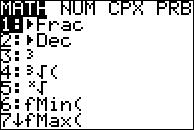
\includegraphics[height=0.7in]{Screen4}
\end{center}
The cube root is listed there, and the general root function below that.  To take the 5th root, for instance, first enter 5, then select that $\sqrt[x]{}$ function, and finally enter the number for which you wish to find the 5th root.
\end{proc}

\begin{example}{Solving Equations with Powers}
Solve the following equation:
\[(x+5)^2 = 36\]

\sol
Now the whole quantity $x+5$ is being squared; just like before, we want to have the squared piece isolated, so that we can take the square root of both sides.

\begin{align*}
(x+5)^2 &= 36\\
\sqrt{(x+5)^2} &= \sqrt{36}\\
x+5 &= 6\\
x &= \boxed{1}
\end{align*}
\end{example}

\subsection{Solving Formulas}

We will often encounter formulas that can be used to calculate some quantity.  For instance, the amount $F$ that a bank account will hold after $t$ years if it earns simple interest at a rate of $r$ and $P$ is deposited today is given by the following formula: \[F = P(1+rt)\]  Each letter in that formula represents a meaningful number (amount deposited, time, etc.).

The way the formula is arranged at first is designed to find $F$ if we are told all the other pieces.  However, we may want to ask the question a different way and look for $P$, the amount we must deposit now in order to reach some goal.  Then $F$ and all the other pieces will be given, and we will need to find $P$.  If we \textbf{solve} the formula for $P$, that will give us an easy way to find $P$ if all the other pieces are given.\\

In other words, when using a formula like the one above, we want to be able to solve for any variable in the formula, in case we want to be able to find a value for that variable if all the other values are known.  The principles for solving a formula are identical to the ones we've seen for solving an equation, except that now we may have to move more variables around.

\begin{example}{Solving Formulas}
Solve for $P$ in the formula below.
\[F = P(1+rt)\]

\sol
As always, we ask the question: what is stopping $P$ from being by itself?  The answer is that it is multiplied by the quantity $(1+rt)$.  Since it is \emph{multiplied}, we can get rid of that by \emph{dividing} both sides of the equation by $(1+rt)$:
\[F = P(1+rt)\]
\[\boxed{\dfrac{F}{1+rt} = P}\]
\end{example}
\pagebreak

\begin{example}{Solving Formulas}
The formula below gives the perimeter $P$ of a rectangle in terms of its length $l$ and width $w$.
\[P = 2(l+w)\]
Solve this formula for $l$.\\

\sol
First, we need to distribute.
\[P = 2l + 2w\]
Then, we will apply the addition and multiplication principles to isolate $l$.
\begin{align*}
P &= 2l + 2w\\
P - 2w &= 2l
\end{align*}

\[\boxed{\dfrac{P-2w}{2} = l}\]
\end{example}

\begin{example}{Solving Formulas}
The formula below describes how to convert a temperature measurement $F$ in terms of degrees Fahrenheit to $C$, given in terms of degrees Celsius.
\[C = \dfrac{5}{9}(F-32)\]
Solve this formula for $F$ (so that the conversion can be done in the other direction).\\

\sol
Here, we first need to divide both sides of the equation by 5/9 in order to start isolating $F$.  Recall that dividing by a fraction (5/9) is the same as multiplying by its reciprocal (9/5).  Therefore, multiplying both sides by 9/5 will remove the fraction from the right side of the formula.
\begin{align*}
C &= \dfrac{5}{9}(F-32)\\
\dfrac{9}{5}C &= F-32
\end{align*}
Now, simply add 32 to both sides to finish solving for $F$.
\[\boxed{F = \dfrac{9}{5}C + 32}\]
\end{example}

\begin{exercises}
\textit{In exercises 1--8, solve each linear equation.}

\pfour{$x+3 = 18$}
\pfour{$4x = 24$}
\pfour{$3x-5 = 4$}
\pfour{$2x-3 = 0$}

\pfour{$2x+9 = 5x$}
\pfour{$6-2y = 3y+1$}
\pfour{$3+2n = 4n+7$}
\pfour{$3(2-x) = 2x-1$}

\textit{In exercises 9--16, solve each equation involving powers.}

\pfour{$x^2 = 25$}
\pfour{$x^3 = -27$}
\pfour{$y^5 = 3125$}
\pfour{$y^2 - 1 = 15$}

\pfour{$x^3 + 3 = 30$}
\pfour{$(x-1)^3 = 64$}
\pfour{$(x+5)^2 = 81$}
\pfour{$(x^2 - 2)^3 = 8$}

\textit{In exercises 17--20, solve each formula for the given variable.}

\ptwo{Electrical power: Solve $P = iV$ for $i$.}
\ptwo{Centripetal force: Solve $F = \dfrac{mv^2}{r}$ for $r$.}

\ptwo{Average of three numbers: Solve $A = \dfrac{a+b+c}{3}$ for $a$.}
\ptwo{Simple interest: Solve $A=P(1+rt)$ for $t$.}

\vspace*{0.25in}

{\color{blue!60!black} \rule{\textwidth}{3pt}}
\vspace*{0.25in}

\subsection{Answers}
\begin{tabularx}{\textwidth}{l l l l l l}
1. $x=15$ & 2. $x=6$ & 3. $x=3$ & 4. $x = 3/2$ & 5. $x=3$ & 6. $y=1$\\ \\
7. $n=-2$ & 8. $x=7/5$ & 9. $x=5,-5$ & 10. $x=-3$ & 11. $y=5$ & 12. $y=4,-4$\\ \\
13. $x=3$ & 14. $x=5$ & 15. $x=4,-14$ & 16. $x=2$ & 17. $i = P/V$ & 18. $r = (mv^2)/F$\\ \\
19. $a=3A-b-c$ & 20. $t=(A-P)/(Pr)$
\end{tabularx}
\end{exercises}